\section*{Dati e risultati}

\subsection*{Transistor come interruttore}

In questa sezione vogliamo verificare il corretto funzionamento del circuito (a).
Il circuito comprende un transistor BC107B, un diodo LED, una resistenza $R_c=1\,\si{\kilo\ohm}$ e una resistenza variabile $R_b$ inizialmente uguale a \SI{100}{\kilo\ohm}. Il circuito è stato alimentato con una tensione costante in ingresso $V\ped{in}$ di $15\,\si{\volt}$.
% non può superare i 15 mA perché ha una resistenza interna di circa 1000 ohm. Se la tensione massima è 15 V il massimo è 15 mA.

Innanzitutto abbiamo verificato che il transistor si comportasse effettivamente come un interruttore, agendo manualmente sull'interruttore (ovvero il cavo banana-banana che collega $R_b$ all'alimentazione). Abbiamo appurato che, scollegando il cavo, il LED non si illumina, mentre se il cavo è collegato, allora il LED è illuminato. Quindi il transistor lascia passare corrente solo se la base è alimentata, come volevamo dimostrare.

Successivamente abbiamo collegato un amperometro tra $R_b$ e il terminale di base del transistor, per misurare $I_b$, e abbiamo misurato $I_e$ con l'alimentatore. In questo modo siamo in grado di osservare come varia la corrente di collettore $I_c = I_e - I_b \simeq I_e$ ($I_b \ll I_e$) al variare della resistenza $R_b$ o della corrente di base $I_b$.

I risultati ottenuti sono riportati nel grafico in Figura \ref{fig:a}

\begin{SCfigure}
    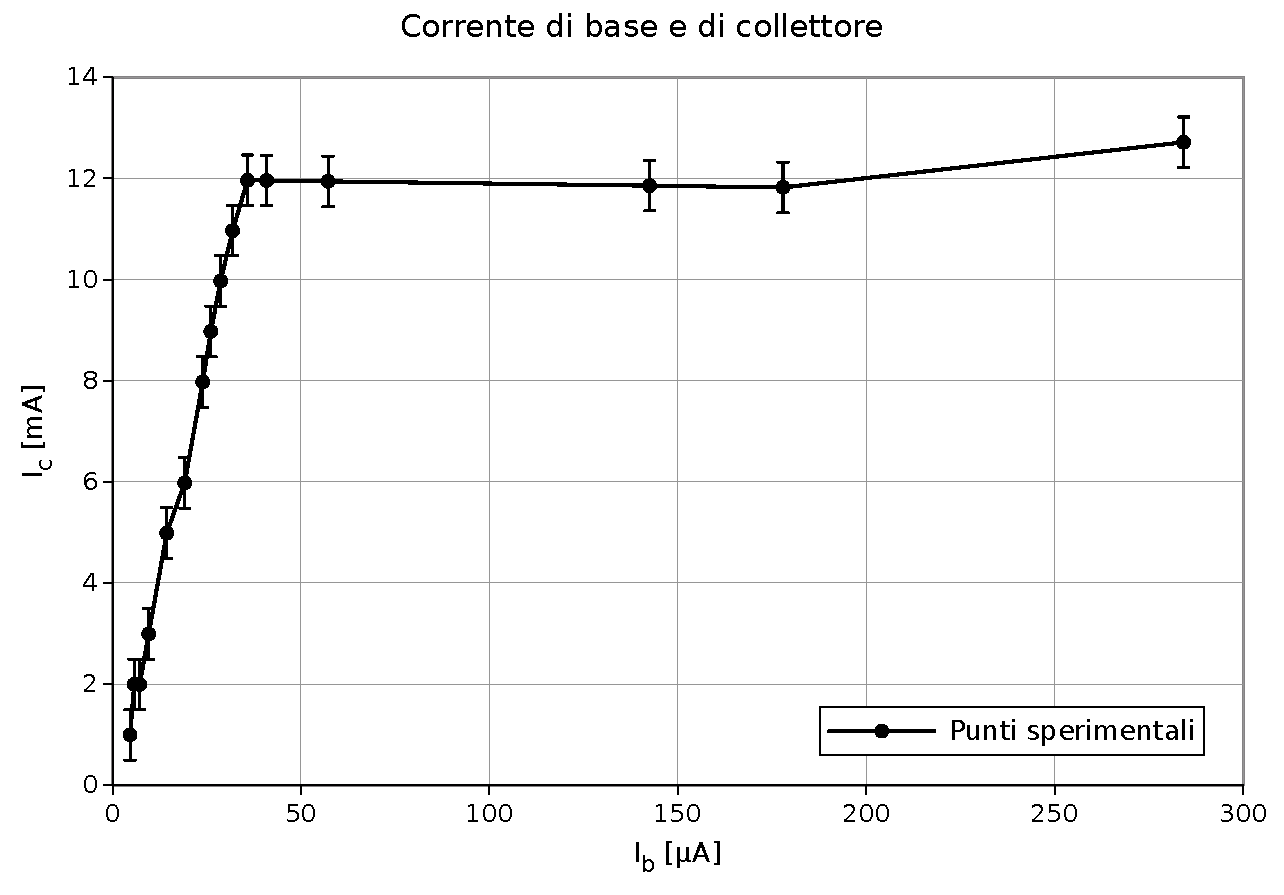
\includegraphics[scale=0.65]{a.pdf}
    \caption{}
    \label{fig:a}
\end{SCfigure}

\subsection*{Transistor come interruttore veloce}

In questa sezione vogliamo verificare che il transistor BC107B, utilizzato nel circuito (b), funzioni effettivamente come interruttore veloce.
Come nel caso precedente la tensione in ingresso $V_0$ è costante ed ha un'intensità di $15\,\si{\volt}$. La resistenza $R_c$ ha un valore di $1\,\si{\kilo\ohm}$ mentre la resistenza $R_b$ vale $10\,\si{\kilo\ohm}$. Inoltre per pilotare il terminale di base del transistor vi abbiamo applicato un segnale in ingresso TTL $V\ped{in}$ fornitoci dal generatore di forme d'onda sotto forma di onda quadra di intervallo $0-5\,\si{\volt}$.

Come abbiamo verificato il transistor utilizzato in questo circuito è effettivamente utilizzabile come interruttore veloce. Infatti fino ad una frequenza massima di circa $20\,\si{\kilo\hertz}$ era possibile distinguere chiaramenti gli intervalli in cui il LED si accendeva e si spegneva. Inoltre per frequenze superiori ai $20\,\si{\kilo\hertz}$  si sarebbe potuto verificare il corretto funzionamento del transistor, come interruttre rapido, utilizzando un fotodiodo[???] con cui avremmo appurato che tale componente è utilizzabile anche con frequenze di circa $15\,\si{\mega\hertz}$, range massimo di funzionamento del nostro generatore di onde.

Il motivo per cui il LED si accende e si spegne è facilmente spiegabile in quanto: il terminale emettitore del transistor si trova ad un potenziale di $0\,\si{\volt}$. Quindi affinche possa passare corrente tra la base e l'emettitore occorre che tra queste vi sia una differenza di potenziale di almeno $0.6\,\si{\volt}$. Quindi dal momento che il segnale in ingresso permette sostanzialmente due valori di tensione di base ($V_b$), ovvero 0 e 5 $\si{\volt}$, allora quando $V_b=0\,\si{\volt}$ il ramo base-emettitore non conduce e nel circuito non passa corrente. Al contrario quando $V_b=5\,\si{\volt}$, allora il ramo base-emettitore entra in conduzione e nel circuito passa corrente e pertanto il LED si illumina.

\subsection*{Emitter follower}

In questa sezione ci proponiamo di montare un circuito emitter follower grazie all'utilizzo di un transistor BC107B nella configurazione illustrata nel circuito (c) . Inoltre vogliamo anche studiare il segnale in uscita ($V\ped{out}$) da tale circuito rispetto al segnale in ingresso al circuito ($V\ped{in}$).

Le specifiche del circuito utilizzato sono le seguenti: il circuito è alimentato con una differenza di tensione in ingresso $V_0$ di $12\,\si{\volt}$, la resistenza $R_b$ ha un valore di $2\,\si{\kilo\ohm}$, la resistenza $R_e$ vale $4.7\,\si{\kilo\ohm}$. Come segnale in ingresso per il terminale di base del transistor abbiamo usato un segnale sinusoidale con una tensione picco-picco effettiva di $10\,\si{\volt}$. Il segnale in ingresso ($V\ped{in}$) è stato generato grazie al generatore di forme d'onda.

I risultati ottenuti sono riportati nel grafico in Figura \ref{fig:}.

\subsection*{}

\subsection*{}
